\documentclass[]{article}
\usepackage{lmodern}
\usepackage{amssymb,amsmath}
\usepackage{ifxetex,ifluatex}
\usepackage{fixltx2e} % provides \textsubscript
\ifnum 0\ifxetex 1\fi\ifluatex 1\fi=0 % if pdftex
  \usepackage[T1]{fontenc}
  \usepackage[utf8]{inputenc}
\else % if luatex or xelatex
  \ifxetex
    \usepackage{mathspec}
  \else
    \usepackage{fontspec}
  \fi
  \defaultfontfeatures{Ligatures=TeX,Scale=MatchLowercase}
\fi
% use upquote if available, for straight quotes in verbatim environments
\IfFileExists{upquote.sty}{\usepackage{upquote}}{}
% use microtype if available
\IfFileExists{microtype.sty}{%
\usepackage{microtype}
\UseMicrotypeSet[protrusion]{basicmath} % disable protrusion for tt fonts
}{}
\usepackage[margin=1in]{geometry}
\usepackage{hyperref}
\hypersetup{unicode=true,
            pdftitle={Numbers Ninja: Class 1},
            pdfborder={0 0 0},
            breaklinks=true}
\urlstyle{same}  % don't use monospace font for urls
\usepackage{color}
\usepackage{fancyvrb}
\newcommand{\VerbBar}{|}
\newcommand{\VERB}{\Verb[commandchars=\\\{\}]}
\DefineVerbatimEnvironment{Highlighting}{Verbatim}{commandchars=\\\{\}}
% Add ',fontsize=\small' for more characters per line
\usepackage{framed}
\definecolor{shadecolor}{RGB}{248,248,248}
\newenvironment{Shaded}{\begin{snugshade}}{\end{snugshade}}
\newcommand{\KeywordTok}[1]{\textcolor[rgb]{0.13,0.29,0.53}{\textbf{#1}}}
\newcommand{\DataTypeTok}[1]{\textcolor[rgb]{0.13,0.29,0.53}{#1}}
\newcommand{\DecValTok}[1]{\textcolor[rgb]{0.00,0.00,0.81}{#1}}
\newcommand{\BaseNTok}[1]{\textcolor[rgb]{0.00,0.00,0.81}{#1}}
\newcommand{\FloatTok}[1]{\textcolor[rgb]{0.00,0.00,0.81}{#1}}
\newcommand{\ConstantTok}[1]{\textcolor[rgb]{0.00,0.00,0.00}{#1}}
\newcommand{\CharTok}[1]{\textcolor[rgb]{0.31,0.60,0.02}{#1}}
\newcommand{\SpecialCharTok}[1]{\textcolor[rgb]{0.00,0.00,0.00}{#1}}
\newcommand{\StringTok}[1]{\textcolor[rgb]{0.31,0.60,0.02}{#1}}
\newcommand{\VerbatimStringTok}[1]{\textcolor[rgb]{0.31,0.60,0.02}{#1}}
\newcommand{\SpecialStringTok}[1]{\textcolor[rgb]{0.31,0.60,0.02}{#1}}
\newcommand{\ImportTok}[1]{#1}
\newcommand{\CommentTok}[1]{\textcolor[rgb]{0.56,0.35,0.01}{\textit{#1}}}
\newcommand{\DocumentationTok}[1]{\textcolor[rgb]{0.56,0.35,0.01}{\textbf{\textit{#1}}}}
\newcommand{\AnnotationTok}[1]{\textcolor[rgb]{0.56,0.35,0.01}{\textbf{\textit{#1}}}}
\newcommand{\CommentVarTok}[1]{\textcolor[rgb]{0.56,0.35,0.01}{\textbf{\textit{#1}}}}
\newcommand{\OtherTok}[1]{\textcolor[rgb]{0.56,0.35,0.01}{#1}}
\newcommand{\FunctionTok}[1]{\textcolor[rgb]{0.00,0.00,0.00}{#1}}
\newcommand{\VariableTok}[1]{\textcolor[rgb]{0.00,0.00,0.00}{#1}}
\newcommand{\ControlFlowTok}[1]{\textcolor[rgb]{0.13,0.29,0.53}{\textbf{#1}}}
\newcommand{\OperatorTok}[1]{\textcolor[rgb]{0.81,0.36,0.00}{\textbf{#1}}}
\newcommand{\BuiltInTok}[1]{#1}
\newcommand{\ExtensionTok}[1]{#1}
\newcommand{\PreprocessorTok}[1]{\textcolor[rgb]{0.56,0.35,0.01}{\textit{#1}}}
\newcommand{\AttributeTok}[1]{\textcolor[rgb]{0.77,0.63,0.00}{#1}}
\newcommand{\RegionMarkerTok}[1]{#1}
\newcommand{\InformationTok}[1]{\textcolor[rgb]{0.56,0.35,0.01}{\textbf{\textit{#1}}}}
\newcommand{\WarningTok}[1]{\textcolor[rgb]{0.56,0.35,0.01}{\textbf{\textit{#1}}}}
\newcommand{\AlertTok}[1]{\textcolor[rgb]{0.94,0.16,0.16}{#1}}
\newcommand{\ErrorTok}[1]{\textcolor[rgb]{0.64,0.00,0.00}{\textbf{#1}}}
\newcommand{\NormalTok}[1]{#1}
\usepackage{graphicx,grffile}
\makeatletter
\def\maxwidth{\ifdim\Gin@nat@width>\linewidth\linewidth\else\Gin@nat@width\fi}
\def\maxheight{\ifdim\Gin@nat@height>\textheight\textheight\else\Gin@nat@height\fi}
\makeatother
% Scale images if necessary, so that they will not overflow the page
% margins by default, and it is still possible to overwrite the defaults
% using explicit options in \includegraphics[width, height, ...]{}
\setkeys{Gin}{width=\maxwidth,height=\maxheight,keepaspectratio}
\IfFileExists{parskip.sty}{%
\usepackage{parskip}
}{% else
\setlength{\parindent}{0pt}
\setlength{\parskip}{6pt plus 2pt minus 1pt}
}
\setlength{\emergencystretch}{3em}  % prevent overfull lines
\providecommand{\tightlist}{%
  \setlength{\itemsep}{0pt}\setlength{\parskip}{0pt}}
\setcounter{secnumdepth}{0}
% Redefines (sub)paragraphs to behave more like sections
\ifx\paragraph\undefined\else
\let\oldparagraph\paragraph
\renewcommand{\paragraph}[1]{\oldparagraph{#1}\mbox{}}
\fi
\ifx\subparagraph\undefined\else
\let\oldsubparagraph\subparagraph
\renewcommand{\subparagraph}[1]{\oldsubparagraph{#1}\mbox{}}
\fi

%%% Use protect on footnotes to avoid problems with footnotes in titles
\let\rmarkdownfootnote\footnote%
\def\footnote{\protect\rmarkdownfootnote}

%%% Change title format to be more compact
\usepackage{titling}

% Create subtitle command for use in maketitle
\newcommand{\subtitle}[1]{
  \posttitle{
    \begin{center}\large#1\end{center}
    }
}

\setlength{\droptitle}{-2em}
  \title{Numbers Ninja: Class 1}
  \pretitle{\vspace{\droptitle}\centering\huge}
  \posttitle{\par}
  \author{Hari Subhash\\
Data Scientist @NRGI}
  \preauthor{\centering\large\emph}
  \postauthor{\par}
  \predate{\centering\large\emph}
  \postdate{\par}
  \date{2018-09-25}


\begin{document}
\maketitle

\subsection{Pre-requisites}\label{pre-requisites}

There two things we need to do before we start the lesson.

\begin{enumerate}
\def\labelenumi{\arabic{enumi}.}
\tightlist
\item
  \href{https://cran.r-project.org/}{Install R}: Any of the links on
  that page should work
\item
  \href{https://www.rstudio.com/products/rstudio/download/}{Install
  Rstudio}: Choose the option that is suited for your Operating System
  (OS).
\end{enumerate}

\subsection{Get familiar with your working
environment}\label{get-familiar-with-your-working-environment}

When you installed R on your computer, you provide it the tools
necessary to process code that is written in R. The Base R installation
ships with a simple code editor that can be used to write R scripts.
RStudio is a software application that builds on top of your R
installation to give you additional functionality to write and manage R
code and projects \footnote{The techinical term for this type of
  software application is:
  \href{https://en.wikipedia.org/wiki/Integrated_development_environment}{integrated
  development environment}(IDE).}. It is by far the most popular
integrated development environment (IDE) for R and has several features
that are custom made to support data science in R.

There are four different panes on RStudio that you need to get familiar
with.

\begin{enumerate}
\def\labelenumi{\arabic{enumi}.}
\tightlist
\item
  The console: This is the pane that is usually located on the left (at
  the bottom if you have a script or notebook open) that can be used to
  type in R commands. The console is a great place to test out lines of
  code that doesn't necessarily have to go into the project you are
  woring on. The console is also the place were the output of your code
  are printed \footnote{This is true for all formats other than those
    that use R Markdown. In the case script formats that use R markdown
    the output is printed within the script rather than in the console.}.
  The console however, is not the place to write any code that you need
  to rerun since it is not possible to save code that is written in the
  console as a file. You will need to use the code pane to do that.
\item
  The code: This is were you will write the majority of the code for
  your projects. There are several different formats in which you can
  write code. This pane only appears if you have an open file that you
  are currently working on. Click on the
  
\includegraphics{assets/scripts.png} button at the top left of R
  Studio to see the different options. We will use the first two options
  R Notebook and R Script for most of this course.
\item
  The viewer: The pane to the bottom right is where you can view plots
  rendered by your code, packages that are currently loaded to the
  environment, access help files, view documents, and access folders on
  your computer. Click on the 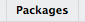
\includegraphics{assets/packages.png} tab
  to scroll through the list and see all the packages that are checked.
  These are the packages that are pre-loaded with your session. If you
  don't know what packages are, don't worry, we will be covering that
  very soon.
\item
  The environment: The environment pane is the one on the top-right.
  This is were all the variables and functions that you create are
  displayed. R Studio provides additional functionality that allows
  users to click on these variables to view their contents. Click on
  
\includegraphics{assets/global environ.png} dropdown you will notice
  that there are several other packages that are listed there. These are
  the same as those that are checked in the packages tab on the viewer
  pane. Selecting one of them will display the entire list of functions
  that are currently available for you to use.
\end{enumerate}

⚡\textbf{\emph{Ninja Tasks}}⚡

\begin{enumerate}
\def\labelenumi{\arabic{enumi}.}
\tightlist
\item
  Create a Numbers Ninja Folder on your local machine
\item
  Create an R Notebook ``Class\_1'' and save it in this folder
\end{enumerate}

\subsection{A quick R Markdown detour}\label{a-quick-r-markdown-detour}

Markdown is a markup language.

\begin{quote}
In computer text processing, a markup language is a system for
annotating a document in a way that is syntactically distinguishable
from the text\ldots{}the whole idea of a mark up language is to avoid
the formatting work for the text, as the tags in the mark up language
serve the purpose to format the appropriate text (like a header or
beginning of a next para\ldots{}etc.). Every tag used in a Markup
language has a property to format the text we write. - Wikipedia
\end{quote}

{Hyper Text Markup
Language}(\href{https://en.wikipedia.org/wiki/HTML}{HTML}) is perhaps
the most well-known markup language out there \footnote{Some other
  examples include - \href{https://en.wikipedia.org/wiki/TeX}{TeX} and
  \href{https://en.wikipedia.org/wiki/LaTeX}{LaTeX}. TeX is the markup
  language that used as a
  \href{https://en.wikipedia.org/wiki/Typesetting}{typesetting system}
  in computers for high quality books. LaTeX is used extensively in
  academia to create documents.}. It is used to render content on
websites. Go ahead and right click on any webpage and click on inspect
to open up the web inspector to view the underlying HTML code that was
used to generate it. {Markdown} is a more human friendly (but limited)
version of HTML. Markdown uses simple and easy to read tags to markup
text which is compiled (by your computer) into HTML that can be used to
render webpages. Making it easier to create content that can be rendered
on a webpage for those who are unfamiliar with HTML.

{R Markdown} is a package in that allows us to combine markdown with R
code. Using R Markdown we can create a wide variety of easy to read and
reproduce R documents that contain both code and nicely formatted. This
online R notebook is a case in point.

In addition to using markdown to markup text, R Markdown documents also
uses {R Markdown}\href{https://en.wikipedia.org/wiki/YAML}{YAML}. This
is the section right at the top of the notebook that is separated by the
\texttt{-\/-\/-}. This is the part of the document were you specify the
title and other characteristics of the report.

Here are a few references to keep handy

\begin{enumerate}
\def\labelenumi{\arabic{enumi}.}
\tightlist
\item
  \href{https://bookdown.org/yihui/rmarkdown/}{R Markdown: The
  definitive guide}
\item
  \href{https://www.rstudio.com/wp-content/uploads/2016/03/rmarkdown-cheatsheet-2.0.pdf}{R
  Markdown cheatsheet}
\end{enumerate}

⚡\textbf{\emph{Ninja Tasks}}⚡

\begin{enumerate}
\def\labelenumi{\arabic{enumi}.}
\tightlist
\item
  Create an H2 level header with title Class 1 Exercises
\item
  Write the following text: ``The list below shows the exercises for
  this class''
\item
  Create an ordered list with following list items: ``1. Practice
  Shortcuts'' ``2. Practice dplyr''
\item
  Click on the preview button at the top left of the IDE to preview your
  notebook
\end{enumerate}

\subsection{Shortcuts}\label{shortcuts}

Before we move on, lets learn a few shortcuts.

\begin{enumerate}
\def\labelenumi{\arabic{enumi}.}
\tightlist
\item
  \texttt{Cmd\ +\ Option\ +\ I} or \texttt{Ctrl\ +\ Alt\ +\ I}: Insert a
  chunk in markdown/notebook etc
\item
  \texttt{Option\ +\ -} or \texttt{Alt\ +\ -}: Enter the assignment
  operator
\item
  \texttt{Cmd\ +\ Enter} or \texttt{Ctrl\ +\ Enter}: Run current
  line/selection
\item
  \texttt{Cmd\ +\ Shift\ +\ Enter} \texttt{Ctrl\ +\ Shift\ +\ Enter}:
  Run the entire script if it is a script file or the current chunk in
  the case of a notebook.
\item
  \texttt{Cmd\ +\ Shift\ +\ M} or \texttt{Ctrl\ +\ Shift\ +\ M}: Insert
  pipe operator
\end{enumerate}

You can find more shortcut keys
\href{https://support.rstudio.com/hc/en-us/articles/200711853-Keyboard-Shortcuts}{here}

⚡\textbf{\emph{Ninja Tasks}}⚡

\begin{enumerate}
\def\labelenumi{\arabic{enumi}.}
\tightlist
\item
  Use all the shortcuts to do the following task: create a new code
  chunk =\textgreater{} assign the string ``Hello World'' to
  \texttt{myFirstVar} variable =\textgreater{} run the line of code
  =\textgreater{} add a print command using \texttt{print(myFirstVar)}
  =\textgreater{} run the entire chunk
\end{enumerate}

\subsection{Packages}\label{packages}

Packages that make our job as coders easier by extending the
functionality of base R. Each package contains a collection of functions
that we can use in our code without having to worry about needing to
write and maintain them ourselves. In addition to functions, packages
can also contain data or point database api (such \texttt{wbstats} which
points to the World Banks data). R has an extremely rich, well
maintained ecosystem of packages that contain functions and data that
are relevant to almost any academic (or even trivial) topics of
interest.

⚡\textbf{\emph{Ninja Tasks}}⚡

\begin{enumerate}
\def\labelenumi{\arabic{enumi}.}
\tightlist
\item
  Install the following packages - \texttt{tidyverse} and
  \texttt{nycflights13} using the package tab in the viewer pane (use
  the 
\includegraphics{assets/install.png} button)
\item
  Use the \texttt{library()} function to load these two packages in the
  Class 1 notebook
\item
  Check the packages tab on your viewer to see if these packages are
  checked (i.e.~loaded to our current environment)
\item
  Check the Global Environment dropdown to see that these are listed.
\end{enumerate}

\subsection{Data Manipulation using
dplyr}\label{data-manipulation-using-dplyr}

The tidyverse We will be using the \texttt{nycflights13} and the
\texttt{tidyverse} packages for this section. Here is a resource to keep
handy whenever you are using the \texttt{tidyverse} for
\href{https://www.rstudio.com/wp-content/uploads/2015/02/data-wrangling-cheatsheet.pdf}{data
wrangling}

\paragraph{Tibbles}\label{tibbles}

⚡\textbf{\emph{Ninja Tasks}}⚡

\begin{enumerate}
\def\labelenumi{\arabic{enumi}.}
\tightlist
\item
  Create a tibble (of your choice) with three observations and three
  variables.
\item
  Show the class and structure of the tibble you created.
\item
  Convert the mtcars data set to a tibble.
\end{enumerate}

🏆\textbf{\emph{Solution}}🏆

Lets create a tibble using the \texttt{tibble()} command. Check out the
code below. Each input in the tibble command is a column. Notice how I
have used both column vectors created within \texttt{tibble()} and an
externally created the vector \texttt{hobby} inside the command.

\begin{Shaded}
\begin{Highlighting}[]
\NormalTok{hobbies <-}\StringTok{  }\KeywordTok{c}\NormalTok{(}\StringTok{"dancing"}\NormalTok{, }\StringTok{"hiking"}\NormalTok{, }\StringTok{"reading"}\NormalTok{)}
\NormalTok{myFavoriteThings <-}\StringTok{ }\KeywordTok{tibble}\NormalTok{(}\DataTypeTok{gadgets =} \KeywordTok{c}\NormalTok{(}\StringTok{"Pixel"}\NormalTok{, }\StringTok{"Kindle"}\NormalTok{, }\StringTok{"Vaccum Cleaner"}\NormalTok{), }\DataTypeTok{books =} \KeywordTok{c}\NormalTok{(}\StringTok{"Das Kapital"}\NormalTok{, }\StringTok{"Harry Potter"}\NormalTok{, }\StringTok{"Enid Blyton"}\NormalTok{), hobbies, }\DataTypeTok{milesRun =} \KeywordTok{c}\NormalTok{(}\DecValTok{1}\NormalTok{, }\DecValTok{3}\NormalTok{, }\DecValTok{10}\NormalTok{))}

\NormalTok{myFavoriteThings}
\end{Highlighting}
\end{Shaded}

\begin{verbatim}
## # A tibble: 3 x 4
##   gadgets        books        hobbies milesRun
##   <chr>          <chr>        <chr>      <dbl>
## 1 Pixel          Das Kapital  dancing        1
## 2 Kindle         Harry Potter hiking         3
## 3 Vaccum Cleaner Enid Blyton  reading       10
\end{verbatim}

Lets checkout the structure using the \texttt{str()} command.

\begin{Shaded}
\begin{Highlighting}[]
\KeywordTok{str}\NormalTok{(myFavoriteThings)}
\end{Highlighting}
\end{Shaded}

\begin{verbatim}
## Classes 'tbl_df', 'tbl' and 'data.frame':    3 obs. of  4 variables:
##  $ gadgets : chr  "Pixel" "Kindle" "Vaccum Cleaner"
##  $ books   : chr  "Das Kapital" "Harry Potter" "Enid Blyton"
##  $ hobbies : chr  "dancing" "hiking" "reading"
##  $ milesRun: num  1 3 10
\end{verbatim}

The tidyverse also provides a function called \texttt{glimpse()} to do
the same thing as \texttt{str()}. Notice the differences between the
outputs from the two commands.

\begin{Shaded}
\begin{Highlighting}[]
\KeywordTok{glimpse}\NormalTok{(myFavoriteThings)}
\end{Highlighting}
\end{Shaded}

\begin{verbatim}
## Observations: 3
## Variables: 4
## $ gadgets  <chr> "Pixel", "Kindle", "Vaccum Cleaner"
## $ books    <chr> "Das Kapital", "Harry Potter", "Enid Blyton"
## $ hobbies  <chr> "dancing", "hiking", "reading"
## $ milesRun <dbl> 1, 3, 10
\end{verbatim}

You can access the class of any object in R using the \texttt{class()}
command. Notice how there are three classes for a tibble - ``tbl\_df'',
``df'' and ``data.frame''. Tibbles really are just data.frames with some
added functionality on top that is provided by the df and tbl\_df
classes.

\begin{Shaded}
\begin{Highlighting}[]
\KeywordTok{class}\NormalTok{(myFavoriteThings)}
\end{Highlighting}
\end{Shaded}

\begin{verbatim}
## [1] "tbl_df"     "tbl"        "data.frame"
\end{verbatim}

\texttt{mtcars} is a part of the \texttt{datasets} package that is
preloaded in R. Lets first look at its structure using \texttt{str()}

\begin{Shaded}
\begin{Highlighting}[]
\KeywordTok{str}\NormalTok{(mtcars)}
\end{Highlighting}
\end{Shaded}

\begin{verbatim}
## 'data.frame':    32 obs. of  11 variables:
##  $ mpg : num  21 21 22.8 21.4 18.7 18.1 14.3 24.4 22.8 19.2 ...
##  $ cyl : num  6 6 4 6 8 6 8 4 4 6 ...
##  $ disp: num  160 160 108 258 360 ...
##  $ hp  : num  110 110 93 110 175 105 245 62 95 123 ...
##  $ drat: num  3.9 3.9 3.85 3.08 3.15 2.76 3.21 3.69 3.92 3.92 ...
##  $ wt  : num  2.62 2.88 2.32 3.21 3.44 ...
##  $ qsec: num  16.5 17 18.6 19.4 17 ...
##  $ vs  : num  0 0 1 1 0 1 0 1 1 1 ...
##  $ am  : num  1 1 1 0 0 0 0 0 0 0 ...
##  $ gear: num  4 4 4 3 3 3 3 4 4 4 ...
##  $ carb: num  4 4 1 1 2 1 4 2 2 4 ...
\end{verbatim}

As you can see the class of mtcars is a data.frame and not a tibble. We
can convert it to a tibble using the \texttt{as\_tibble()} command.
Below, I have used this command to create a new tibble called
\texttt{mtTibble}. The output shows it structure. Notice that now we
have the two additional classes ``df'' and ``tbl\_df'' that characterize
tibbles.

\begin{Shaded}
\begin{Highlighting}[]
\NormalTok{mtTibble <-}\StringTok{ }\KeywordTok{as_tibble}\NormalTok{(mtcars)}

\KeywordTok{str}\NormalTok{(mtTibble)}
\end{Highlighting}
\end{Shaded}

\begin{verbatim}
## Classes 'tbl_df', 'tbl' and 'data.frame':    32 obs. of  11 variables:
##  $ mpg : num  21 21 22.8 21.4 18.7 18.1 14.3 24.4 22.8 19.2 ...
##  $ cyl : num  6 6 4 6 8 6 8 4 4 6 ...
##  $ disp: num  160 160 108 258 360 ...
##  $ hp  : num  110 110 93 110 175 105 245 62 95 123 ...
##  $ drat: num  3.9 3.9 3.85 3.08 3.15 2.76 3.21 3.69 3.92 3.92 ...
##  $ wt  : num  2.62 2.88 2.32 3.21 3.44 ...
##  $ qsec: num  16.5 17 18.6 19.4 17 ...
##  $ vs  : num  0 0 1 1 0 1 0 1 1 1 ...
##  $ am  : num  1 1 1 0 0 0 0 0 0 0 ...
##  $ gear: num  4 4 4 3 3 3 3 4 4 4 ...
##  $ carb: num  4 4 1 1 2 1 4 2 2 4 ...
\end{verbatim}

\paragraph{The Pipe Operator}\label{the-pipe-operator}

\begin{Shaded}
\begin{Highlighting}[]
\NormalTok{mtcars[[}\DecValTok{3}\NormalTok{]]}
\end{Highlighting}
\end{Shaded}

\begin{verbatim}
##  [1] 160.0 160.0 108.0 258.0 360.0 225.0 360.0 146.7 140.8 167.6 167.6
## [12] 275.8 275.8 275.8 472.0 460.0 440.0  78.7  75.7  71.1 120.1 318.0
## [23] 304.0 350.0 400.0  79.0 120.3  95.1 351.0 145.0 301.0 121.0
\end{verbatim}

\begin{Shaded}
\begin{Highlighting}[]
\NormalTok{models <-}\StringTok{ }\NormalTok{mtcars }\OperatorTok\StringTok{ }
\StringTok{  }\KeywordTok{split}\NormalTok{(.}\OperatorTok{$}\NormalTok{cyl) }\OperatorTok\StringTok{ }
\StringTok{  }\KeywordTok{map}\NormalTok{(}\ControlFlowTok{function}\NormalTok{(df) }\KeywordTok{lm}\NormalTok{(mpg }\OperatorTok{~}\StringTok{ }\NormalTok{wt, }\DataTypeTok{data =}\NormalTok{ df))}

\NormalTok{models }\OperatorTok\StringTok{ }
\StringTok{  }\KeywordTok{map}\NormalTok{(summary) }\OperatorTok\StringTok{ }
\StringTok{  }\KeywordTok{map_dbl}\NormalTok{(}\OperatorTok{~}\NormalTok{.}\OperatorTok{$}\NormalTok{r.squared)}
\end{Highlighting}
\end{Shaded}

\begin{verbatim}
##         4         6         8 
## 0.5086326 0.4645102 0.4229655
\end{verbatim}

⚡\textbf{\emph{Ninja Tasks}}⚡

\begin{enumerate}
\def\labelenumi{\arabic{enumi}.}
\tightlist
\item
  Calculate the square root of the sum of all even numbers from 0 to 200
  and create a sequence that goes from the square root to twice its
  value.
\end{enumerate}

\begin{Shaded}
\begin{Highlighting}[]
\KeywordTok{seq}\NormalTok{(}\DataTypeTok{from =} \DecValTok{1}\NormalTok{, }\DataTypeTok{to =} \DecValTok{100}\NormalTok{, }\DataTypeTok{by =} \DecValTok{2}\NormalTok{) }\OperatorTok\StringTok{ }
\StringTok{        }\KeywordTok{sum}\NormalTok{() }\OperatorTok\StringTok{ }
\StringTok{        }\KeywordTok{sqrt}\NormalTok{() }\OperatorTok\StringTok{ }
\StringTok{        }\KeywordTok{seq}\NormalTok{(}\DataTypeTok{from =}\NormalTok{ ., }\DataTypeTok{to =}\NormalTok{ .}\OperatorTok{*}\DecValTok{3}\NormalTok{, }\DataTypeTok{by =} \DecValTok{3}\NormalTok{)}
\end{Highlighting}
\end{Shaded}

\begin{verbatim}
##  [1]  50  53  56  59  62  65  68  71  74  77  80  83  86  89  92  95  98
## [18] 101 104 107 110 113 116 119 122 125 128 131 134 137 140 143 146 149
\end{verbatim}

\begin{Shaded}
\begin{Highlighting}[]
\KeywordTok{seq}\NormalTok{(}\DataTypeTok{from =} \KeywordTok{sqrt}\NormalTok{(}\KeywordTok{sum}\NormalTok{(}\KeywordTok{seq}\NormalTok{(}\DataTypeTok{from =} \DecValTok{1}\NormalTok{, }\DataTypeTok{to =} \DecValTok{100}\NormalTok{, }\DataTypeTok{by =} \DecValTok{2}\NormalTok{))), }\DataTypeTok{to =} \DecValTok{3} \OperatorTok{*}\StringTok{ }\KeywordTok{sqrt}\NormalTok{(}\KeywordTok{sum}\NormalTok{(}\KeywordTok{seq}\NormalTok{(}\DataTypeTok{from =} \DecValTok{1}\NormalTok{, }\DataTypeTok{to =} \DecValTok{100}\NormalTok{, }\DataTypeTok{by =} \DecValTok{2}\NormalTok{))), }\DataTypeTok{by =} \DecValTok{3}\NormalTok{)}
\end{Highlighting}
\end{Shaded}

\begin{verbatim}
##  [1]  50  53  56  59  62  65  68  71  74  77  80  83  86  89  92  95  98
## [18] 101 104 107 110 113 116 119 122 125 128 131 134 137 140 143 146 149
\end{verbatim}

\paragraph{Filter}\label{filter}

Lets find all the flights that departed in the morning

\begin{Shaded}
\begin{Highlighting}[]
\NormalTok{morningFlights <-}\StringTok{ }\NormalTok{flights }\OperatorTok\StringTok{ }
\StringTok{        }\KeywordTok{filter}\NormalTok{(dep_time }\OperatorTok{<=}\StringTok{ }\DecValTok{1200} \OperatorTok{&}\StringTok{ }\NormalTok{month }\OperatorTok{==}\StringTok{ }\DecValTok{1} \OperatorTok{&}\StringTok{ }\NormalTok{day }\OperatorTok{==}\StringTok{ }\DecValTok{1}\NormalTok{)}

\KeywordTok{max}\NormalTok{(morningFlights}\OperatorTok{$}\NormalTok{dep_time, }\DataTypeTok{na.rm =}\NormalTok{ T)}
\end{Highlighting}
\end{Shaded}

\begin{verbatim}
## [1] 1200
\end{verbatim}

The most delayed flight from JFK in 2013

\begin{Shaded}
\begin{Highlighting}[]
\NormalTok{flights }\OperatorTok\StringTok{ }
\StringTok{        }\KeywordTok{filter}\NormalTok{(origin }\OperatorTok{==}\StringTok{ "EWR"}\NormalTok{) }\OperatorTok\StringTok{ }
\StringTok{        }\KeywordTok{filter}\NormalTok{(dep_delay }\OperatorTok{==}\StringTok{ }\KeywordTok{max}\NormalTok{(dep_delay, }\DataTypeTok{na.rm =}\NormalTok{ T))}
\end{Highlighting}
\end{Shaded}

\begin{verbatim}
## # A tibble: 1 x 19
##    year month   day dep_time sched_dep_time dep_delay arr_time
##   <int> <int> <int>    <int>          <int>     <dbl>    <int>
## 1  2013     1    10     1121           1635      1126     1239
## # ... with 12 more variables: sched_arr_time <int>, arr_delay <dbl>,
## #   carrier <chr>, flight <int>, tailnum <chr>, origin <chr>, dest <chr>,
## #   air_time <dbl>, distance <dbl>, hour <dbl>, minute <dbl>,
## #   time_hour <dttm>
\end{verbatim}

\begin{Shaded}
\begin{Highlighting}[]
\KeywordTok{max}\NormalTok{(flights}\OperatorTok{$}\NormalTok{dep_delay, }\DataTypeTok{na.rm =}\NormalTok{ T)}
\end{Highlighting}
\end{Shaded}

\begin{verbatim}
## [1] 1301
\end{verbatim}

⚡\textbf{\emph{Ninja Tasks}}⚡

\begin{enumerate}
\def\labelenumi{\arabic{enumi}.}
\tightlist
\item
  Which flight out of JFK was the most delayed in 2013?
\end{enumerate}

\begin{Shaded}
\begin{Highlighting}[]
\KeywordTok{library}\NormalTok{(nycflights13)}


\NormalTok{flights }\OperatorTok\StringTok{ }
\StringTok{    }\KeywordTok{filter}\NormalTok{(origin }\OperatorTok{==}\StringTok{ "JFK"}\NormalTok{) }\OperatorTok\StringTok{ }
\StringTok{    }\KeywordTok{filter}\NormalTok{(dep_delay }\OperatorTok{==}\StringTok{ }\KeywordTok{max}\NormalTok{(dep_delay, }\DataTypeTok{na.rm =}\NormalTok{ T))}
\end{Highlighting}
\end{Shaded}

\begin{verbatim}
## # A tibble: 1 x 19
##    year month   day dep_time sched_dep_time dep_delay arr_time
##   <int> <int> <int>    <int>          <int>     <dbl>    <int>
## 1  2013     1     9      641            900      1301     1242
## # ... with 12 more variables: sched_arr_time <int>, arr_delay <dbl>,
## #   carrier <chr>, flight <int>, tailnum <chr>, origin <chr>, dest <chr>,
## #   air_time <dbl>, distance <dbl>, hour <dbl>, minute <dbl>,
## #   time_hour <dttm>
\end{verbatim}

\begin{enumerate}
\def\labelenumi{\arabic{enumi}.}
\setcounter{enumi}{1}
\tightlist
\item
  Answer the previous question without using dplyr or pipes.
\end{enumerate}

\begin{Shaded}
\begin{Highlighting}[]
\NormalTok{jfkFlights <-}\StringTok{ }\NormalTok{flights[flights}\OperatorTok{$}\NormalTok{origin }\OperatorTok{==}\StringTok{ "JFK"}\NormalTok{, ]}

\NormalTok{maxDelay <-}\StringTok{ }\KeywordTok{max}\NormalTok{(jfkFlights}\OperatorTok{$}\NormalTok{dep_delay, }\DataTypeTok{na.rm =}\NormalTok{ T)}

\NormalTok{jfkFlights[jfkFlights}\OperatorTok{$}\NormalTok{dep_delay }\OperatorTok{==}\StringTok{ }\NormalTok{maxDelay }\OperatorTok{&}\StringTok{ }\OperatorTok{!}\KeywordTok{is.na}\NormalTok{(jfkFlights}\OperatorTok{$}\NormalTok{dep_delay), ]}
\end{Highlighting}
\end{Shaded}

\begin{verbatim}
## # A tibble: 1 x 19
##    year month   day dep_time sched_dep_time dep_delay arr_time
##   <int> <int> <int>    <int>          <int>     <dbl>    <int>
## 1  2013     1     9      641            900      1301     1242
## # ... with 12 more variables: sched_arr_time <int>, arr_delay <dbl>,
## #   carrier <chr>, flight <int>, tailnum <chr>, origin <chr>, dest <chr>,
## #   air_time <dbl>, distance <dbl>, hour <dbl>, minute <dbl>,
## #   time_hour <dttm>
\end{verbatim}

\begin{enumerate}
\def\labelenumi{\arabic{enumi}.}
\setcounter{enumi}{2}
\tightlist
\item
  What were the 5 longest flights (in air time) from NYC in 2013?
\end{enumerate}

\begin{Shaded}
\begin{Highlighting}[]
\NormalTok{flights }\OperatorTok
\StringTok{    }\KeywordTok{arrange}\NormalTok{(}\KeywordTok{desc}\NormalTok{(air_time)) }\OperatorTok\StringTok{ }
\StringTok{    }\KeywordTok{filter}\NormalTok{(}\KeywordTok{row_number}\NormalTok{() }\OperatorTok{<=}\StringTok{ }\DecValTok{5}\NormalTok{)}
\end{Highlighting}
\end{Shaded}

\begin{verbatim}
## # A tibble: 5 x 19
##    year month   day dep_time sched_dep_time dep_delay arr_time
##   <int> <int> <int>    <int>          <int>     <dbl>    <int>
## 1  2013     3    17     1337           1335         2     1937
## 2  2013     2     6      853            900        -7     1542
## 3  2013     3    15     1001           1000         1     1551
## 4  2013     3    17     1006           1000         6     1607
## 5  2013     3    16     1001           1000         1     1544
## # ... with 12 more variables: sched_arr_time <int>, arr_delay <dbl>,
## #   carrier <chr>, flight <int>, tailnum <chr>, origin <chr>, dest <chr>,
## #   air_time <dbl>, distance <dbl>, hour <dbl>, minute <dbl>,
## #   time_hour <dttm>
\end{verbatim}

another easier way to do this

\begin{Shaded}
\begin{Highlighting}[]
\NormalTok{flights }\OperatorTok\StringTok{ }
\StringTok{    }\KeywordTok{top_n}\NormalTok{(air_time, }\DataTypeTok{n =} \DecValTok{5}\NormalTok{)}
\end{Highlighting}
\end{Shaded}

\begin{verbatim}
## # A tibble: 5 x 19
##    year month   day dep_time sched_dep_time dep_delay arr_time
##   <int> <int> <int>    <int>          <int>     <dbl>    <int>
## 1  2013     2     6      853            900        -7     1542
## 2  2013     3    15     1001           1000         1     1551
## 3  2013     3    16     1001           1000         1     1544
## 4  2013     3    17     1006           1000         6     1607
## 5  2013     3    17     1337           1335         2     1937
## # ... with 12 more variables: sched_arr_time <int>, arr_delay <dbl>,
## #   carrier <chr>, flight <int>, tailnum <chr>, origin <chr>, dest <chr>,
## #   air_time <dbl>, distance <dbl>, hour <dbl>, minute <dbl>,
## #   time_hour <dttm>
\end{verbatim}

\paragraph{Select}\label{select}

\begin{Shaded}
\begin{Highlighting}[]
\NormalTok{flights }\OperatorTok\StringTok{ }
\StringTok{    }\KeywordTok{filter}\NormalTok{(origin }\OperatorTok\StringTok{ }\KeywordTok{c}\NormalTok{(}\StringTok{"JFK"}\NormalTok{)) }\OperatorTok\StringTok{ }\NormalTok{##origin == "JFK" | origin == "EWR"}
\StringTok{    }\KeywordTok{select}\NormalTok{(origin, }\KeywordTok{contains}\NormalTok{(}\StringTok{"dest"}\NormalTok{),air_time) }\OperatorTok\StringTok{ }
\StringTok{    }\KeywordTok{top_n}\NormalTok{(air_time, }\DataTypeTok{n =} \DecValTok{10}\NormalTok{)}
\end{Highlighting}
\end{Shaded}

\begin{verbatim}
## # A tibble: 10 x 3
##    origin dest  air_time
##    <chr>  <chr>    <dbl>
##  1 JFK    HNL        667
##  2 JFK    HNL        669
##  3 JFK    HNL        675
##  4 JFK    HNL        679
##  5 JFK    HNL        691
##  6 JFK    HNL        676
##  7 JFK    HNL        686
##  8 JFK    HNL        683
##  9 JFK    HNL        686
## 10 JFK    HNL        671
\end{verbatim}

⚡\textbf{\emph{Ninja Tasks}}⚡

\begin{enumerate}
\def\labelenumi{\arabic{enumi}.}
\tightlist
\item
  Select all the columns that are relevant for arrival and departure
  delays using a utility function (refer to cheat sheet)
\end{enumerate}

\paragraph{Arrange}\label{arrange}

\begin{Shaded}
\begin{Highlighting}[]
\NormalTok{flights }\OperatorTok\StringTok{ }
\StringTok{    }\KeywordTok{arrange}\NormalTok{(}\KeywordTok{desc}\NormalTok{(dep_delay))}
\end{Highlighting}
\end{Shaded}

\begin{verbatim}
## # A tibble: 336,776 x 19
##     year month   day dep_time sched_dep_time dep_delay arr_time
##    <int> <int> <int>    <int>          <int>     <dbl>    <int>
##  1  2013     1     9      641            900      1301     1242
##  2  2013     6    15     1432           1935      1137     1607
##  3  2013     1    10     1121           1635      1126     1239
##  4  2013     9    20     1139           1845      1014     1457
##  5  2013     7    22      845           1600      1005     1044
##  6  2013     4    10     1100           1900       960     1342
##  7  2013     3    17     2321            810       911      135
##  8  2013     6    27      959           1900       899     1236
##  9  2013     7    22     2257            759       898      121
## 10  2013    12     5      756           1700       896     1058
## # ... with 336,766 more rows, and 12 more variables: sched_arr_time <int>,
## #   arr_delay <dbl>, carrier <chr>, flight <int>, tailnum <chr>,
## #   origin <chr>, dest <chr>, air_time <dbl>, distance <dbl>, hour <dbl>,
## #   minute <dbl>, time_hour <dttm>
\end{verbatim}

Hypothesis: Flights are more delayed around Christmas. Compare
mean(dep\_delay) to find the answer.

Find the answer? Is that correct?

⚡\textbf{\emph{Ninja Tasks}}⚡

\begin{enumerate}
\def\labelenumi{\arabic{enumi}.}
\tightlist
\item
  Filter the top 10 most delayed flights in JFK and arrange by
  dep\_delay (highest to lowest)
\end{enumerate}

\paragraph{Mutate}\label{mutate}

⚡\textbf{\emph{Ninja Tasks}}⚡

\begin{enumerate}
\def\labelenumi{\arabic{enumi}.}
\tightlist
\item
  Create a new variable called total\_delay that is the sum of the
  arrival delay and departure delay
\end{enumerate}

\paragraph{Group and Summarise}\label{group-and-summarise}

⚡\textbf{\emph{Ninja Tasks}}⚡

\begin{enumerate}
\def\labelenumi{\arabic{enumi}.}
\tightlist
\item
  Create a summary table with the following characteristics for each of
  the origin airports.

  \begin{itemize}
  \tightlist
  \item
    Number of flights
  \item
    Number of unique carriers
  \item
    Average departure delays
  \item
    Average flight times (air time)
  \item
    Average arrival delays
  \end{itemize}
\end{enumerate}

⚡\textbf{\emph{Ninja Tasks}}⚡

\subsection{Post-requisites}\label{post-requisites}

\begin{enumerate}
\def\labelenumi{\arabic{enumi}.}
\tightlist
\item
  Setup a \href{https://github.com}{GitHub Account}
\item
  Install \href{https://desktop.github.com/}{GitHub Desktop}
\item
  Read up about
  \href{https://www.atlassian.com/git/tutorials/what-is-version-control}{version
  control}
\item
  Read up about the
  \href{https://cran.r-project.org/web/packages/tidyverse/vignettes/manifesto.html}{tidy
  tools manifesto}
\end{enumerate}


\end{document}
